\documentclass[11pt]{report}
\usepackage{unhthesis}
\usepackage{graphics}
\usepackage{longtable}

%------------------------------------------------------------------------------
%  Preliminary Pages - Fill in the `blanks' noted.
%------------------------------------------------------------------------------

\begin{document}
			% TITLE PAGE
							%======================
\title{DETERMINISTIC EXECUTION IN A JAVA-LIKE LANGUAGE} % Your title
\author{Niels Widger}					% Your name
\prevdegrees{B.S., University of New Hampshire (2009)}	% Your old degree
\major{Computer Science}				% Your new major
\degree{Master of Science}				% Your new degree
\degreemonth{Januart}					% When awarded.
\degreeyear{2014}					%
\thesisdate{\today}					% Date of document.
\DOCUMENTtype{THESIS}				% or DISSERTATION
\Documenttype{Thesis}				% or Dissertation
\documenttype{thesis}				% or dissertation
\maketitle
							% COPYRIGHT PAGE
							%======================
%\copyrightyear{2007}					% Delete these
%\makecopyright						% if no copyright
							% page.

							% APPROVAL PAGE
							%======================
\supervisor{Philip Hatcher,}{Professor of Computer Science}
\committee{Michel Charpentier,}{Associate Professor of Computer Science}
\committee{Robert Russell,}{Associate Professor of Computer Science}
\makeapproval						%

			% ACK. PAGE
							%======================
\begin{acknowledgments}
  I would like to thank Professor Hatcher for all of his help
  throughout this entire project.  I would also like to thank my
  committee for their guidance and advice.
\end{acknowledgments}


			% OTHER PAGES
							%======================
\tableofcontents					% Always needed...
\listoftables						% Delete if no tables.
\addcontentsline{toc}{section}{LIST OF TABLES}
\listoffigures						% Delete if no figures.
\addcontentsline{toc}{section}{LIST OF FIGURES}

%------------------------------------------------------------------------------
%  Document body - Place text into individual include files, such as
%                  as "chap1.tex", or replace each "\include{}" statement
%                  with your actual document text.
%------------------------------------------------------------------------------

%% begin code environment
\newcommand{\bnncode}{
	\begin{tabbing}
	00. nn\=nn\=nn\=nn\=nn\=nn\=nn\=nn\=nn\=nn\kill
}

%% end code environment
\newcommand{\ecode}{\end{tabbing}}

\newcounter{lnctr}
\setcounter{lnctr}{0}
\newcommand{\codeln}{%
  \addtocounter{lnctr}{1}%
  \arabic{lnctr}}

			% ABSTRACT PAGE
							%======================
\begin{abstractpage}
  Nondeterministic execution makes multithreaded programming
  difficult.  Nondeterministic execution causes programs to produce
  different output given the same input, makes concurrency bugs
  difficult to reproduce and makes unit testing less conclusive.
  Recent research has shown that deterministic execution of parallel
  programs can be achieved with overhead small enough that it is
  sufficient for debugging purposes and perhaps even for deployment.
  Previous work has focused on deterministic execution of arbitrary
  C/C++ code by instrumenting the code with calls into a run-time
  framework.  My thesis instead focused on executing a Java-like
  language deterministically by implementing deterministic execution
  inside the virtual machine.  I believed that differences in the
  memory model, instruction set and architecture will allow
  deterministic execution of a Java-like language to be done with
  lower overhead than a C-like language.
\end{abstractpage}


\pagenumbering{arabic}
			% CHAPTERS
							%======================
\chapter{INTRODUCTION}

Nondeterministic execution is an unfortunate side effect of existing
multicore and multiprocessor systems.  Nondeterminism in parallel
programs can arise from many different factors such as differences in
thread scheduling, cache state and I/O delays.  Nondeterministic
execution leads to an array of problems:

\begin{itemize}
\item it causes programs to produce different output when executed
  with the same inputs

\item makes concurrency bugs such as race conditions hard to reproduce

\item creates bugs that lie dormant in multithreaded code for years
  before an input and thread interleaving are executed that causes
  them to be discovered

\item makes unit testing of multithreaded code difficult and less
  conclusive

\item causes major frustrations to programmers wishing to enjoy the
  benefits of parallel programming
\end{itemize}

However, recent research has shown that deterministic execution of
parallel programs is possible on today's hardware, and can be achieved
with overhead small enough that it is sufficient for debugging
purposes and, depending on the application, even for deployment.

A program is said to execute deterministically if it always produces
the same output given the same inputs.  Deterministic execution offers
several advantages such as more reliable testing, reproducible bugs
and more useful crash reports.  The overhead required to ensure
deterministic execution can be reduced if certain assumptions about
the program are made.  Strong determinism guarantees a deterministic
ordering of all shared memory accesses for a given input.  Weak
determinism guarantees a deterministic ordering of all lock
acquisitions for a given input.  Weak determinism yields deterministic
execution only if the program is data-race free, while strong
determinism makes no assumptions about program correctness.  Strong
determinism is concerned with all accesses to shared memory whereas
weak determinism requires that only lock operations are watched.
Because of this, the overhead to enforce strong determinism is higher
than weak determinism.

Most research in deterministic execution has been in the form of
run-time frameworks for C/C++ code that requires code to be recompiled
before it can be executed deterministically.  In contrast, my thesis
involved applying existing deterministic execution techniques to a
Java-like language that is executed in a virtual machine.  I believed
is that these techniques can be applied with lower overhead in a
virtual machine setting than in a compiled language.

%%% Local Variables: 
%%% mode: latex
%%% TeX-master: "thesis"
%%% End: 

\chapter{BACKGROUND}
\label{BACKGROUND}

There has been significant work on deterministic execution in the
literature.  In this section, we highlight several different
techniques and give a brief overview of their strengths and
weaknesses.

\section{Deterministic Shared Memory Multiprocessing (DMP)}

Devietti et al.\ describe a method of executing a multithreaded
program with a strong deterministic guarantee that they call
deterministic shared memory multiprocessing (DMP)~\cite{dmp}.
Previous work on deterministic execution focused on deterministic
replay systems that have high overheads due to their need to record a
log of the ordering of events that can then be replayed for debugging
purposes~\cite{recplay}.  In contrast, DMP enforces deterministic
execution dynamically as the program executes.

As they describe in their paper, a naive way to achieve deterministic
execution is to ensure that the interleaving of every instruction is
exactly the same for every execution.  One way to do this is to
serialize execution such that only one thread is allowed to execute at
a time.  Each thread is allowed to execute only if it holds the
\emph{deterministic token}.  By allowing each thread to execute some
deterministic number of instructions, called a \emph{quantum}, while
holding the token and by enforcing a deterministic order in which each
thread receives the deterministic token, deterministic execution is
achieved.  In their paper, they refer to a \emph{round} as one cycle
in which each thread executes a single quantum.

Serializing the entire program as described above defeats the
performance advantages of programming using threads.  In their paper,
Devietti et al.\ make the point that if two instructions do not
communicate, the order in which they execute is irrelevant~\cite{dmp}.
Therefore, deterministic execution can be achieved by carefully
controlling only those instructions that cause interthread
communication via shared memory.  By controlling the order in which
load/store instructions to shared memory execute, each dynamic
instance of a load instruction can be made to always read data from
the same dynamic instance of a store instruction.

Using this idea, and keeping the concepts of rounds, quanta and a
deterministic token, parallelism can be recovered by allowing threads
to execute in parallel so long as they do not communicate.  To do
this, each quantum is broken into two modes: \emph{parallel mode} and
\emph{serial mode}.  In parallel mode, all threads execute
concurrently.  Each thread executes in parallel mode until either:

\begin{itemize}
\item It reaches the end of its quantum.

\item It attempts to access a memory location that may cause
  interthread communication.
\end{itemize}

At the start of each round, all threads execute the parallel segment
of the current quantum and block waiting for serial mode to begin when
one of the above conditions is met.  Serial mode begins after all
threads have finished executing their parallel segment.  Once this
occurs, execution is serialized by passing the deterministic token and
allowing each thread to run their serial segment in isolation.  At
this time, each thread is allowed unrestricted access to shared memory
(both reads and writes).  For each thread, serial mode ends once they
execute the remainder of their quantum (which may be empty, if the
first condition marks the end of their parallel segment).  When a
thread finishes executing its serial segment, it passes the
deterministic token to the next thread and blocks waiting for serial
mode to end.  After each thread finishes executing its serial segment,
a new round begins with each thread executing the parallel segment of
the next quantum.

Determinism in DMP is guaranteed on the same input for the following
reasons:

\begin{itemize}
\item No interthread communication can occur during parallel mode as
  it is detected and deferred until serial mode.

\item Each thread's parallel segment will end at a deterministic point
  because, given the same input, a thread will always follow the same
  execution path leading to either the first or second condition being
  met.

\item Serial mode is deterministic because threads are executed
  serially in a deterministic order.
\end{itemize}

In their paper, the deterministic token is passed in thread creation
order from oldest to youngest.  Thread creation and destruction are
deferred until serial mode.  Newly created threads are placed at the
end of the deterministic execution order but do not begin executing
until parallel mode.

All threads in the same process have access to the same shared memory
space.  Therefore, it might seem that any access to shared memory
should be detected as possible interthread communication.  However, in
practice threads often store private data in this same memory space
that is never accessed by other threads.  A thread accessing its own
private data should not have to block for serial mode.  Similarly, it
is common for shared data to be accessed in a read-only manner amongst
several threads.  A thread should not have to block to read shared
read-only data as this cannot cause nondeterminism.

Therefore, in order to accurately detect that interthread
communication is about to occur via a read/write to shared memory, the
ownership/sharing state of each memory location must be tracked.  To
do this, a global \emph{ownership table} is maintained that, for each
memory location, tracks its shared state and, if the memory location
is not shared, its current owner.  The granularity of each entry in
the ownership table can be of any size such as byte-, word- or
page-level.  Choosing a size involves a trade-off between accuracy and
performance.  A memory location can either be shared amongst all
threads or privately owned by a single thread.  Before executing each
load/store instruction to shared memory, the ownership table is
consulted and the instruction is either allowed to execute or the
thread is made to block for serial mode.  An \emph{ownership table
  policy} defines the following:

\begin{itemize}
\item When an entry in the ownership table transitions between being
  marked as shared or private.

\item When the ownership of an entry in the ownership table
  transitions from one thread to another.

\item When a thread executing in parallel mode is allowed to proceed
  with a memory access.
\end{itemize}

\begin{table}
  \begin{tabular}{l|l|l|l}
    owned  &  sh/priv  &  rd/wr    &  action                         \\
    \hline
    yes    &  priv     &  -        &  proceed                        \\
    -      &  sh       &  rd       &  proceed                        \\
    -      &  sh       &  wr       &  block, set priv+owned, proceed \\
    no     &  priv     &  rd       &  block, set sh, proceed         \\
    no     &  priv     &  wr       &  block, set priv+owned, proceed \\
  \end{tabular}
  \caption{Ownership table policy used in DMP paper}
  \label{table:ownership-policy}
\end{table}

Table~\ref{table:ownership-policy} summarizes the ownership table
policy used by DMP~\cite{dmp}.  Note that during serial mode, while a
thread does not need to block to access a memory location, the
transitions between shared and private in the table still occur.  The
ownership status of a memory location is only relevant if the memory
location is marked as private in the ownership table.  If a memory
location is private, only the thread marked as its owner is allowed to
access it during parallel mode.  All other threads must block for
serial mode to access that location.  A thread becomes the owner of a
memory location marked as private when it writes to that location in
serial mode after blocking.  This policy ensures that a thread does
not have to block to access its own private data, and also ensures
that changes to private data by its owner are made visible to other
threads at a deterministic point in time, i.e. during serial mode.
Figure~\ref{fig:ownership-graph} shows the possible state transitions
for a memory location accessible by two threads $t$ and $u$.

\begin{figure}[!]
  \begin{center}
    {\resizebox{3.10in}{!}{
        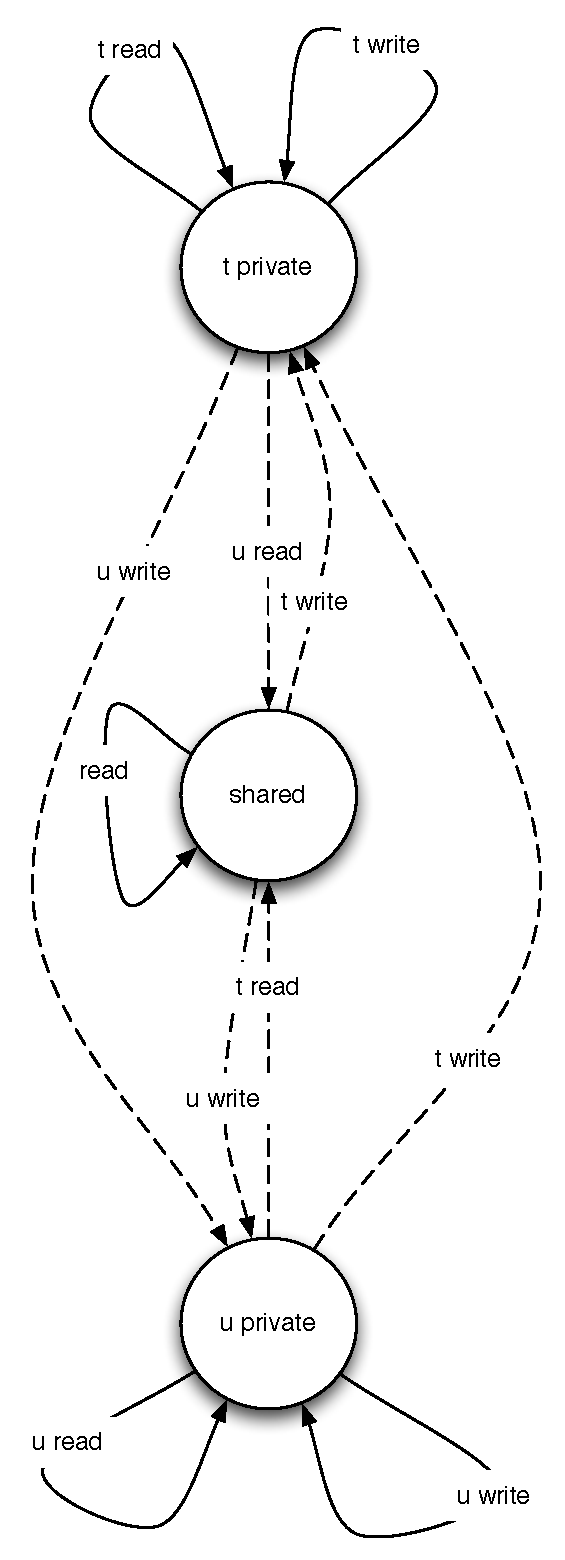
\includegraphics{./figures/ownership-graph.pdf} }}
  \end{center}
  \vspace{-4mm}
  \caption{Ownership transition graph for a memory location accessible to two
    threads.}
  \label{fig:ownership-graph}
\end{figure}

In order to improve the performance of data shared in a read-only
manner, when a memory location marked as private is read by a thread
that is not its owner, that memory location transitions to being
marked as shared.  A memory location marked as shared has no owner.
While it is marked as shared, any thread can read that memory location
during parallel mode without blocking, but writes can only be made in
serial mode.  A memory location marked as shared transitions back to
being marked as private when a thread blocks and writes to it in
serial mode, and in doing so becomes its owner.

During parallel mode, a thread is allowed full access to memory marked
as private that it owns and read-only access to memory marked as
shared.  For all other accesses, a thread must first block for serial
mode.  Note that during parallel mode, the ownership table is strictly
read-only.  A thread is only allowed to modify the ownership table
during serial mode.  Therefore, no synchronization of the ownership
table is needed because during serial mode only one thread may be
executing at a time.

To see that the above policy makes sense, first consider a policy that
considers the ``owned'' column of Table~\ref{table:ownership-policy}
but ignores the ``shared/private'' and ``read/write'' columns.  Under
such a policy, a thread can access a memory location in parallel mode
only if it is the current owner, therefore ensuring determinism as no
interthread communication can occur.  Next, add the ``shared/private''
and ``read/write'' columns back into the policy.  Now a thread can
access a memory location in parallel mode if it is the current owner
or if it is shared and the access is a read.  This change does not
affect determinism because a shared memory location cannot be written
to by any thread until serial mode, therefore a read access during
parallel mode cannot cause nondeterminism.  Transfer of ownership and
transitions between shared and private are performed after a thread
has blocked for serial mode and are done in an attempt to take
advantage of the principle of locality.  If a thread is likely to
access a memory location again, it is logical to modify the ownership
table such that its next access will not cause it to block.  However,
any policy for modifying the shared/private status of a memory
location during serial mode is acceptable so long as it is
deterministic.

As mentioned previously, quanta can be constructed using any policy so
long as it is deterministic.  In their paper, Devietti et al.\ discuss
several policies for constructing quanta~\cite{dmp}.  They refer to
these as \emph{quantum building policies}.  They experiment with
several different policies:

\begin{itemize}
\item Each quantum lasts until $N$ instructions have been performed.

\item Each quantum lasts until an unlock operation is performed.

\item Each quantum lasts until $N$ consecutive accesses to memory
  marked as private have been performed.

\item Boolean $OR$ of the second and third policies.
\end{itemize}

The first policy is the simplest to implement and simply locks a
quantum down to a fixed size.  The second and third policies try to
detect when a thread has left a critical section, hopefully marking
the end of a period of interthread communication.  In their paper,
Devietti et al.\ also experiment with two styles of serial
mode~\cite{dmp}:

\begin{itemize}
\item Serial mode lasts until the end of the quantum.

\item Serial mode lasts until the end of the quantum or until the
  thread performs an unlock operation and the thread is not holding
  any other locks.
\end{itemize}

They refer to the first style as \emph{full serial mode} and the
second style as \emph{reduced serial mode}.  Reduced serial mode is an
attempt to end serial mode at the end of a critical section in which
interthread communication occurs.

For a given round, the ideal quantum building policy would result in
the parallel segments of each thread being precisely the same length
and the serial segments of each thread being zero-length.  A quantum
in which each parallel segment is precisely the same length is called
\emph{balanced} and is ideal because it minimizes the amount of time
each thread blocks waiting for serial mode.  A quantum with a
zero-length serial mode is ideal because it minimizes serialization.
In practice, most programs will not have a zero-length serial mode as
there will be a varying amount of interthread communication.
Therefore, the question of how long serial mode should be comes into
question.  If serial mode is too short, a thread with many consecutive
shared memory accesses may not be able to complete them all in its
serial segment and may block too soon into its next parallel segment,
likely leading to imbalance.  If serial mode is too long, parallelism
is reduced by making the execution too serialized.

Devietti et al.\ argue that deterministic execution should be used not
only for debugging but should be left on when the product is deployed.
Their paper advocates for a change in multiprocessor system
architecture such that deterministic execution using the methods
described are implemented in hardware.  In their implementation, they
use the cache line state maintained by a MESI cache coherence protocol
to track ownership status.  To evaluate their ideas, they simulate a
hardware implementation of DMP using PIN, a program analysis tool.

There are both advantages and disadvantages to the DMP method of
deterministic execution.  DMP makes no assumptions about the behavior
of the program.  Other frameworks require a program be data-race free
in order to guarantee determinism.  However, it is important to note
that DMP will always execute a program such that communicating
instructions are interleaved in the same order.  DMP does not control
non-communicating instructions, which may be interleaved or may occur
simultaneously in any order.  Two executions in which all
communicating instructions are ordered the same are known as
\emph{communication-equivalent interleavings}.

If the particular set of communication-equivalent interleavings that
DMP generates reveals a bug, that bug will occur every time the
program is executed.  This makes it easy to fix concurrency bugs that
surface when the program is run with a given input.  However, testing
a program with DMP can only guarantee that the program is bug-free
when run using that input and when run using the thread interleavings
generated by DMP.  It is possible that other bugs exist but do not
surface with the particular set of interleavings DMP allows.  This is
a definite disadvantage of DMP.  If the overhead of leaving DMP on
when deploying a product is too large, a product might be extensively
tested with DMP across a wide range of inputs, but miss bugs that only
surface after the product is deployed with DMP turned off.  Therefore,
to be most effective the overhead of DMP must be small enough that it
can be left on across the life of the product.

Their experimental results show that deterministic execution can be
achieved with acceptable performance using DMP implemented in
hardware.  Hardware DMP using an ownership table incurred a slowdown
of between 37\% and 15\%.

\section{CoreDet}

CoreDet is an implementation of DMP in software.  Bergan et al.\ use a
modified LLVM C/C++ compiler with several new compiler phases that add
instrumentation code before load and store instructions to shared
memory~\cite{coredet}.  The instrumentation code calls into the
CoreDet run-time framework that consults an in-memory ownership table
and decides if the instruction can be executed immediately or must
wait for serial mode.  The ownership table and all other data
structures needed by the framework is stored in global shared memory.
A major contribution of CoreDet is that it shows that DMP can be
implemented effectively in software and it extends the original DMP
paper by adding two new approaches to deterministic execution.

The first approach drops the use of a global ownership table to
prevent uncontrolled interthread communication.  Instead, each thread
has a local store buffer that caches writes to shared memory made
during parallel mode.  When a thread reads a location, it first
consults its store to see if it has a modified value for that location
and otherwise retrieves the value from global shared memory.  This
means that shared memory is read-only during parallel mode.  Writes
cached in a thread's store buffer are committed to global shared
memory in a new commit mode that occurs between parallel mode and
serial mode.  A clever algorithm allows most commits to be made in
parallel while still preserving the deterministic commit order.  This
is done by allowing threads to commit in parallel while maintaining
enough metadata to prevent one thread's writes from overwriting some
other thread that comes after it in the deterministic commit order.
By using a store buffer, the need to block for serial mode is greatly
reduced.  Parallel mode ends when either of the following conditions
hold:

\begin{itemize}
\item A memory fence instruction is reached.

\item An atomic operation such as a compare-and-swap must be
  performed.
\end{itemize}

The second approach combines ownership tracking with the store buffer.
The global ownership table is brought back and is maintained the same
as in the original DMP paper, thus allowing distinction of accesses to
shared data from accesses to private data.  While in parallel mode, a
thread can access its own private data without blocking and without
consulting its local store, but accesses to another thread's private
data must wait until serial mode.  If a thread wishes to access shared
data while in parallel mode, it must consult its local store.  This
second approach reduces the overhead incurred by the frequent
consulting of the store buffer that the original approach suffers
from.

For their evaluation, they implement three versions of DMP: one using
the ownership table introduced in the original DMP paper, a second
using a store buffer and a third using a combination of both.  Their
results show that the ownership table has low overhead but limited
scalability as execution becomes more serialized as the number of
threads is increased.  The store buffer implementation offers good
scalability but higher overhead due to the high cost required to
access and maintain the store buffer.  The performance of using both
the ownership table and a store buffer is somewhere in between the
first two in terms of scalability and overhead.

\section{Kendo}

Kendo is a software framework that offers a weak determinism guarantee
for lock-based, data-race free C/C++ code.  Olszewski, Ansel, and
Amarasinghe guarantee determinism using Kendo for data-race free
programs by guaranteeing a deterministic order of all lock
acquisitions for a given program input~\cite{kendo}.  Kendo implements
a subset of the POSIX Threads API, replacing the existing
synchronization functions (such as $pthread\_mutex\_lock$,
$pthread\_mutex\_unlock$, etc.) with calls to their own run-time
framework.  Programs run using Kendo must first be recompiled and
linked with the Kendo run-time framework.

In order to achieve its goal of weak determinism, each thread
maintains a \emph{deterministic logical clock} that is incremented
deterministically, potentially after every instruction.  Each lock
stores the deterministic logical clock of the last thread to release
the lock.  In their basic algorithm, a thread attempting to acquire
the lock must wait until all threads with smaller thread ID's have
greater deterministic logical clock and all threads with larger thread
ID's have greater or equal deterministic logical clocks.  Using these
rules, Kendo maintains the invariant that only one thread may hold a
lock at a given logical time in order to guarantee determinism.

Kendo is an effective and fairly lightweight method of guaranteeing
deterministic execution, however in order to guarantee determinism it
requires that a program be data-race free.  A program will not execute
deterministically using Kendo unless all shared data is protected by a
consistent set of locks.  This hurts its usefulness, especially in
debugging parallel programs, as having a deterministic guarantee while
trying to debug a multithreaded program is one of the main goals of
deterministic execution.

\section{Grace}

Grace is a run-time framework that enables safe and efficient
concurrent programming.  Programs executed using Grace are said to be
\emph{behaviorally equivalent} to their sequential counterparts.  This
means a program executed using Grace will produce the same output as
the original program executed with thread spawns converted to regular
function invocations.  The order in which functions would be invoked
in this single-threaded version is known as \emph{program order}.
Grace is designed for fork-join parallelism applications in which a
parent function spawns one or more children and then waits for them to
terminate before returning itself.  Berger et al.\ designed Grace in
an attempt to get rid of a large number of concurrency bugs while
still achieving good performance~\cite{grace}.  The concurrency bugs
that Grace eliminates and their causes are:

\begin{itemize}
\item Deadlocks - cyclic lock acquisition.

\item Race conditions - unguarded updates.

\item Atomicity violations - unguarded, interleaved updates.

\item Order violations - threads scheduled in unexpected order.
\end{itemize}

Grace achieves its goal by allowing multiple threads to execute
simultaneously, but executes each thread in a separate transaction
such that they are isolated and appear to execute atomically.  Grace
prevents a thread from committing its transaction to shared memory
until all of its logical predecessors have committed successfully.  In
the case of a parent spawning one or more children, this means a
parent cannot commit until all of its children have committed.  In the
case of a child thread, this means it cannot commit until all of its
siblings who were spawned earlier by its parent have committed.  Grace
eliminates the above sources of concurrency bugs in the following
manner:

\begin{itemize}
\item No deadlocks - all lock acquisitions/releases are converted to
  no-ops.

\item No race conditions - all transactions commit changes to shared
  memory in a deterministic order.

\item No atomicity violations - all threads execute atomically in an
  isolated transaction.

\item No order violations - threads are executed in program order.
\end{itemize}

Grace uses virtual memory-based software transactional memory to allow
concurrent execution of multiple threads while still ensuring that
execution is behaviorally equivalent to a serial execution.  To do
this, each memory location stores a version number that is incremented
whenever it is updated.  Using the operating system's virtual memory
facilities, each thread is given two mappings of shared memory: a
shared mapping that reflects the last successful commit and a private
copy-on-write mapping used for local changes.  As a thread executes,
it maintains a read-set and write-set containing the memory locations
that it read from and wrote to, respectively.  When a thread is ready
to terminate, it must commit all changes in its write-set to shared
memory.  To do this, it checks the committed versions numbers to those
in its read set.  If they match, the commit is allowed.  Otherwise,
the thread aborts as its calculations were performed on out-of-date
data.  The thread must abort and be re-executed using the new memory
space.

Because threads commit in program order, Grace is designed for
applications with many small, short-running threads such that threads
do not wait very long before they can commit. Because Grace runs
threads in isolation using transactions, Grace is restricted to a
subset of parallel applications.  For instance, Berger et
al.~\cite{grace} note that the following thread behaviors are not
supported:

\begin{itemize}
\item Threads that run infinitely or until program is terminated.

\item Threads that perform interthread communications (i.e., via
  synchronization primitives such as condition variables).
\end{itemize}

This means that Grace cannot work as a general solution to
deterministic execution.

\section{Deterministic Parallel Java}

Deterministic Parallel Java (DPJ) is an extension to the Java
programming language that adds parallel code blocks as well as a
\emph{type and effect} system that allows a compile-time guarantee of
determinism~\cite{dpj}.  DPJ splits the heap into named
\emph{regions}.  DPJ source code is annotated to indicate in which
region a data member is allocated.  Similarly, method definitions are
annotated to indicate which regions they read and which regions they
write (known as \emph{read effects} and \emph{write effects}).  The
region into which each object is allocated is computed at
compile-time.  Using the annotations in the source code, provided by
the programmer, the DPJ compiler determines if a given program will
execute deterministically.  This is done by ensuring that all pairs of
memory accesses are either both reads, access disjoint regions of the
heap or are properly synchronized to prevent concurrent access.

DPJ uses compile-time enforcement of determinism, meaning its overhead
at run-time is very small when compared to other solutions such as
DMP.  However, it could be argued that the type and effect systems
used by DPJ is clumsy and frustrating to the programmer.  The
annotations that must be provided by the programmer can wind up being
very complicated and hard to understand.  Furthermore, determinism can
only be guaranteed if every annotation is correct, and the burden to
fix any inaccuracies is placed on the programmer's shoulders.

\section{maTe DMP}

My thesis is that a Java-like programming language can be executed
deterministically using DMP with less overhead than a C-like
programming language.  A Java-like language is object-oriented where
objects are accessed through references, is byte-compiled and is
executed in a virtual machine.  A C-like language contains primitive
data-types, pointers and is compiled to native code.  In my research,
I modified maTe, a Java-like language, and used it to test my thesis.
I built upon existing work in the area of deterministic execution to
implement DMP inside the maTe virtual machine using quanta and an
ownership tracking system.

As described earlier, DMP relies on an ownership tracking mechanism to
maintain the shared/private status of each memory location in shared
memory in order to detect interthread communication that can cause
nondeterminism.  When detected, execution of each thread is serialized
for a small period of time so that communication is performed in a
deterministic order.  The ownership table policy determines how memory
locations transition between shared/private during serial mode.  This
policy is important not only because it is used to enforce determinism
but also because it has a large effect on performance.  For example, a
policy that relies only on thread ownership will yield worse
performance than a policy that also takes into account private/shared
status and whether the access is a read or write.

The key idea of my thesis is that, in a Java-like language where
shared memory can only be accessed through object references, the
ability of a thread to access a memory location can be determined at
any point by traversing the global object graph.  Compare this to
C-like languages where, through the use of pointers, arbitrary memory
locations can be accessed and no memory location can be truly
considered private.  While escape analysis at compile-time can
determine that an object is thread local, it cannot prevent the use of
unsafe memory operations at run-time.  Therefore any ownership
tracking technique used in such a language must be conservative.

Executing inside of a virtual machine also offers advantages to
deterministic execution.  In the Java virtual machine, each method
frame has its own local variable array and operand stack that are
private and cannot be accessed by other threads (or even other methods
executing in the same thread).  Therefore, instructions that operate
on these locations need not be instrumented, reducing overhead.  The
same cannot be said of C, in which a thread's stack is located in
shared memory space.

\begin{figure}[!]
  \begin{center}
    {\resizebox{\textwidth}{!}{
        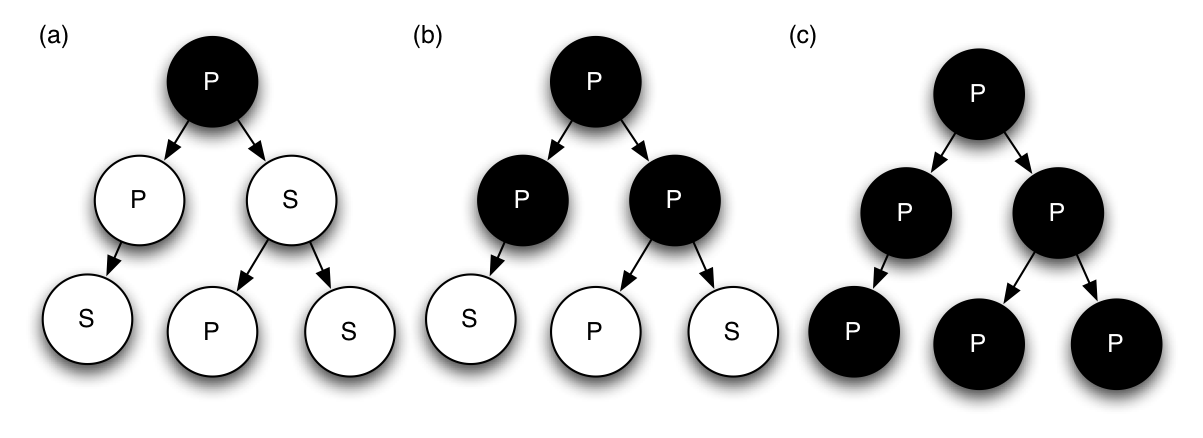
\includegraphics{./figures/depth.png} }}
  \end{center}
  \caption{Example of changes in ownership due to a write using depth 1 (a), 2
    (b) and 3 (c).}
  \label{fig:depth}
\end{figure}

As mentioned earlier, large chunks of memory can be privatized quickly
by choosing a large granularity for the ownership table.  This is done
in the hope of avoiding the need to block to access nearby memory in
the future.  In a C-like language, two memory locations are ``nearby''
if their addresses in memory are nearby.  ``Nearby'' has a different
meaning in a Java-like language as there is no concept of addresses.
Instead, the relative distance between two objects is computed by
finding the shortest path between them in the global object graph.
Therefore, in my implementation, the granularity of the ownership
table is given not in units of bytes, words or pages but in depth.  At
a depth of one, only the ownership table entry of the object being
accessed is modified, at a depth of two, the object being modified as
well as all objects it reference are modified and so on.
Figure~\ref{fig:depth} illustrates the changes in object ownership
that occur when writing to the object at the root of the tree using an
ownership table depth of 1, 2 and 3.  Blackened objects are those
marked as private and owned by the writing thread.

In order to test my thesis, I extended the maTe programming language
and implemented DMP using an ownership table in the maTe virtual
machine.  I did not implement the local store buffer used by
CoreDet~\cite{coredet}.  maTe is a pure object-oriented,
byte-compiled, garbage-collected programming language.  maTe features
support for single inheritance, virtual method calls, method and
operator overloading, nested local variable declarations and basic
input/output facilities.  maTe includes no primitive data types.
Instead, maTe includes four predefined classes to allow for integer
arithmetic, text manipulation and simple data storage: Object,
Integer, String and Table (Table is a key/value pair hash map inspired
by Java's $java.util.HashMap$ class).

Grammatically, maTe source is very similar to Java source code.  An
example of maTe source code can be seen in Figure~\ref{fig:mate-code}.
maTe source code is translated by the maTe compiler to an intermediate
maTe assembly language before being assembled by the maTe assembler
into a platform independent binary class file.  Class files are
executed inside the maTe virtual machine, which implements the maTe
instruction set as well as the predefined classes in native code.

\begin{figure}[!]
\begin{small}
  \small \bnncode
  \codeln. class Point \{ \\
  \codeln. \> Integer x, y; \\
  \codeln. \> Point(Integer x, Integer y) \{ this.x = x; this.y = y; \} \\
  \codeln. \> Point operator+(Point p) \{ return new Point(x + p.x, y + p.y); \} \\
  \codeln. \> Integer equals(Object obj) \{ \\
  \codeln. \>\> if (obj == null) return 0; \\
  \codeln. \>\> if (obj instanceof Point) \{ \\
  \codeln. \>\>\> Point p; \\
  \codeln. \>\>\> p = (Point)obj; \\
  \codeln. \>\>\> if (x.equals(p.x) \&\& y.equals(p.y)) \{ \\
  \codeln. \>\>\>\> return 1; \\
  \codeln. \>\>\> \} \\
  \codeln. \>\> \} \\
  \codeln. \>\> return 0; \\
  \codeln. \> \} \\
  \codeln. \> String toString() \{ return "(" + x.toString() + ", " + y.toString() + ")"; \} \\
  \codeln.  \} \\
  \codeln. Integer main() \{ \\
  \codeln. \> Point p, q, r; \\
  \codeln. \> p = new Point(10, 10); \\
  \codeln. \> q = new Point(5, 5); \\
  \codeln. \> r = p + q; \\
  \codeln. \> out "p = " + p.toString() + newline; \\
  \codeln. \> out "q = " + q.toString() + newline; \\
  \codeln. \> out "r = " + r.toString() + newline; \\
  \codeln. \> return 0; \\
  \codeln. \}
  \ecode \vspace{-0mm}
  \caption{\label{fig:mate-code} Example of maTe source code.}
\end{small}
\end{figure}

Architecturally, the maTe virtual machine is modeled after the Java
virtual machine.  Method frames are stored on a global stack with each
method frame holding a local variable array and operand stack.  The
local variable array stores arguments and local variables.  The
operand stack stores parameters to be passed to methods and receives
method results.  Upon startup, the class file to be executed is loaded
into memory and an in-memory version of the class table is generated.
Memory for new objects is allocated from a global heap.  The maTe
instruction set is also modeled after Java.  It uses high level
instructions that allows implementation of much of the method
dispatch/stack maintenance to be pushed up to the virtual machine
instead of being handled by the compiler.

The current implementation of the maTe language is done in a mix of C
and C++.  The assembler and virtual machine are implemented in C while
the compiler is written in C++ using flex/bison as the scanner/parser
generator.  The maTe virtual machine includes a conservative
concurrent, snapshot-at-the-beginning garbage collector implemented
using the tri-color abstraction and a mark stack.  The garbage
collector is run in a separate thread using the $pthreads$ threading
library.

%%% Local Variables: 
%%% mode: latex
%%% TeX-master: "thesis"
%%% End: 

\chapter{IMPLEMENTATION}
\label{IMPLEMENTATION}

\section{maTe Language}

Originally, the maTe language only allowed for integer arithmetic
using the predefined Integer class.  I added a new predefined class,
Real, that wraps a float primitive to allow scientific applications
that require floating point calculations to be written.

In order to test multithreaded programs, the maTe language was
modified to support user-created threads.  I used Java's threading
model as a guide in creating a new predefined $Thread$ class.  Users
extend this class and override the $run$ method that is called after
the user begins execution of the thread with a call to its $start$
method.

In order to allow for critical sections and synchronization, a monitor
in the form of a mutex was added to each object in the virtual
machine.  An object's monitor can be acquired and released using new
$monitorenter$ and $monitorexit$ instructions.  The language was
extended to allow for synchronized blocks, the body of which is
executed only after acquiring the monitor of a particular object.
Three new methods were added to the base Object class: $wait$,
$notify$ and $notifyAll$ adding support for asynchronous events.
These new methods function entirely similarly to those in Java.  A
thread can block for another thread to terminate by calling the $join$
method on a particular $Thread$ instance or block for a specific
length of time using the $sleep$ method.

These changes to the language required modifications to all of the
development tools.  The grammar of the language used by the compiler
was be modified to include synchronized blocks.  At code generation
time, the compiler emits the new $monitorenter$ and $monitorexit$
instructions at the entrance and exit of each synchronized block.
Corner cases involving $break$ or $return$ statements inside nested
synchronized blocks had to be accounted for.  To do so, the compiler
was modified to maintain a monitor stack to ensure that all currently
acquired monitors are released regardless of the execution path.  The
assembler was modified to be aware of the new instructions and their
respective opcodes.

I also added support for $for$ loops, boolean operators $\&\&$ and
$\|\|$ and $!=$, $<=$ and $>=$ operators to the compiler.  None of
these changes impacted the assembler or virtual machine, however they
did make implementing the benchmarks much easier.

\section{maTe Virtual Machine}

The majority of the changes required to test this thesis were made in
the virtual machine.  This step can be broken down into two parts:
implementing threads and implementing DMP.

\subsection{Implementing Threads}

The first step was adding support for multiple user threads in the
virtual machine.  Each $Thread$ instance is allocated a virtual
machine stack and is executed using the $pthreads$ threading library.
Because a $Thread$ instance cannot be collected while its $run$ method
is still executing, regardless of its accessibility via the global
object graph, $Thread$ instances are protected from the garbage
collector by adding them to a global thread set whose contents are not
considered for deletion by the garbage collector.  The garbage
collector also uses this set to iterate over the stack of each thread
while marking the roots during its mark phase.  Finally, a
$pthread\_mutex\_t$ accessed by the new $monitorenter$ and
$monitorexit$ instructions was added to each object created by the
virtual machine.

Initially, additional synchronization through the use of mutexes were
added to many of the virtual machine's data structures such as the
heap, stack and stack frame.  However, in order to increase
performance when running multiple threads, many of these mutexes were
eliminated.

\subsection{Implementing DMP}

The second and largest step was implementing DMP inside the virtual
machine.  As describe earler, there are four situations that can cause
a thread to block when DMP is enabled:

\begin{itemize}
\item upon executing a communicating $getfield$ or $putfield$
  instruction (used to read/write an object field),
\item upon creation of a $Thread$ instance (by calling its $start$
  method),
\item upon termination of the $run$ method of a $Thread$ instance, and
\item upon reaching the end of its quantum in the fetch/execute loop
\end{itemize}

The implemention must satisfy these requirements.  In addition, I had
a number of architectural goals in mind when implementing DMP:

\begin{itemize}
\item be able to enable/disable DMP using a command-line argument
  without needing to compile the maTe source code,
\item isolate DMP functionality into separate files with minimal hooks
  in the main virtual machine implementation,
\item minimize any performance penalty caused by DMP implementation
  when running with DMP disabled and
\item allow the possibility for DMP behavior to be per-thread or
  per-object specific.
\end{itemize}

In order to achieve these goals, a new DMP-specific module was created
for the $object$, $table$, $thread$ and $nlock$ modules.  Each module
stores a pointer to the respective DMP-specific module, and a $NULL$
pointer check is placed before a hook into the DMP-specific module is
called to determine if DMP is enabled on that module.  Therefore, when
running with DMP disabled, these modules store one extra pointer field
and must perform a handful of extra pointer comparisons but their
performance and behavior is otherwise unchanged.

The $nlock$ module implements the mutex used by the $monitorenter$ and
$monitorexit$ instructions and wraps operations performed on the
$pthread\_mutex\_t$ used by each object.  A DMP-specific module for
$nlock$ is needed for two reasons.  First, the virtual machine needs
to track monitors acquired by a thread in order to implement reduced
serial mode.  Secondly, with DMP enabled the virtual machine must use
non-blocking system calls when trying to acquire a mutex to ensure a
thread does not stall indefinitely while waiting for a mutex.  This
situation can occur when a thread tries to acquire a mutex held by
another thread during its turn in serial mode or in parallel mode when
it is the last thread to block.

% figure illustrating pointer to DMP module for object, perhaps
% showing some of the function names.

A single instance of the global $dmp$ module is created when the
virtual machine starts up.  The DMP-specific modules for $object$,
$table$, $thread$ and $nlock$ are allocated through this module.  In
addition, this module holds the $barrier$ instance used to synchronize
threads between parallel/serial mode.  The $barrier$ module was
implemented using a $pthread\_mutex\_t$ mutex and $pthread\_cond\_t$
condition variable.  Threads call into the $dmp$ module at the end of
their current segment with a call to $dmp\_thread\_block$.  In
parallel mode, the $dmp$ module ensures each thread blocks until the
end of the current parallel segment.  In serial mode, the $dmp$ module
wakes each thread in creation order and ensures all other threads are
blocked.  Finally, the $dmp$ module implements the default ownership
table policy for shared memory reads/writes.  Before allowing a
$getfield$ or $putfield$ to actually read/write an object's field, the
DMP-specific $object$ module passes in the ID of the object it is
going to access.  The $dmp$ module returns a $thread$ action ($block$
or $proceed$) and an $owner$ action ($none$, $set shared$ or $set
private$) to perform.

The DMP-specific modules were designed to be very flexible.  Each
module is passed a set of attributes at creation time.  These
attributes include an operations table as well as any
settings/counters needed by the module.  Although the functionality
was not implemented, it would be possible to give certain
objects/threads different attributes, containing different operations
tables or metadata based on any arbitrary policy.  A feature such as
this could be used to implement a kind of ``fuzz testing'' scenario in
which a program is repeatedly executed with different DMP attributes
for each object/thread in an attempt to discover concurrency bugs
uncovered by certain thread interleavings.

The heap stores a set containing all $Thread$ instances sorted by
creation time.  This is used to wake each thread in a deterministic
order so that it can execute its serial segment.  Upon reaching the
end of its serial segment, each thread calls the global barrier again.
After all threads have reached the second barrier, a new round begins
with all threads executing in parallel.

The parallel garbage collector implemented in the virtual machine
posed for deterministic execution since when a collection cycle would
occur is not deterministic.  Therefore, only the serial garbage
collector is used when running with DMP enabled.  The garbage
collector is run at the end of serial mode if the heap is using $90\%$
or more of its maximum memory.

\subsubsection{Object DMP}

The default $object$ attributes are $owner$, the thread ID of the
object's current owner, and $depth$, the ownership table granularity
used by the object.  The entries in the operations table correspond to
DMP operations handled by that module.  The DMP-specific $object$
module has three operations: $load$, $store$ and $chown$.  The $load$
and $store$ operations allow the module to block the thread based on
an attempt to read/write a given object (by calling into the $dmp$
module), and $chown$ implements propagating any ownership changes
based on the ownership table depth.  A default action is executed if a
pointer in the operations table is $NULL$.

The ownership table is not stored as a global data structure but
instead distributed amongst all objects using the DMP-specific
$object$ module's $owner$ attribute.  If $owner$ is $0$, the object is
shared.  If $owner$ is not $0$, the object is private and the value
specifies the thread ID of its current owner.  The DMP-specific
$thread$ module maintains an executed instructions count to track the
end of its quantum which is incremented for each iteration of the
fetch/execute loop.  Hooks into the DMP-specific $object$ module were
placed into the $object$ module's $object\_load\_field$ and
$object\_store\_field$ functions (which are called from the $getfield$
and $putfield$ instructions).  The default $load$ and $store$
operations follow the ownership table policy from the DMP paper by
checking the $owner$ field before allowing the instruction to execute.

\subsubsection{Thread DMP}

The DMP-specific $thread$ module has four attributes: the serial mode
(full/reduced) being used by the thread, the number of locks currently
held by the thread, the quantum size and the number of instructions
executed by the thread in the current quantum.  The operations table
has six entries: $thread\_creation$, $thread\_start$,
$thread\_destruction$, $thread\_join$ and
$thread\_execute\_instruction$.  The $thread\_creation$ entry is
called in $Thread.start$ and prevents a new thread from being created
until serial mode.  The $thread\_start$ entry is called at the very
top of $Thread.run$ and ensures the thread sleeps until its turn in
serial mode.  The $thread\_destruction$ entry is called at the very
end of $Thread.run$ and waits until the next parallel segment before
destroying the thread.  The $thread\_join$ entry is called in
$Thread.join$ and causes the thread to block for parallel/serial mode
if the thread it is waiting on has not terminated yet.  This must be
done to prevent a deadlock if a thread tries to join a thread that has
already blocked waiting for the next parallel/serial mode.  The
$thread\_execute\_instruction$ entry is called each time a thread
executes an opcode and ensures the thread blocks once it has executed
as many instructions as is dictated by its quantum size.

\subsubsection{Table DMP}

The DMP-specific $table$ module is perhaps the strangest of all the
DMP-specific modules.  The operations table has only two entries:
$load$ and $store$.  The $Table$ object has no object fields since it
is entirely implemented within the virtual machine.  The internal
state of a $Table$ instance is accessible from a maTe program only
through method calls.  The purpose of the DMP-specific $table$ module
is to ensure that threads accessing the native fields of a $Table$
instance blocks appropriately just as it would be it were accessing a
maTe object field.  The default $load$ and $store$ implementations
merely call the $load$ and $store$ operations of the $Table$
instance's DMP-specific $object$ module.

\subsubsection{NLock DMP}

The DMP-specific $nlock$ module prevents the virtual machine from
losing control of a thread when it blocks waiting to acquire an
object's monitor.  The DMP-specific $nlock$ operations table has three
entries: $lock$, $unlock$ and $timedwait$.  The default $lock$
implementation continually causes a thread to block until the thread
will successfully acquire the monitor.  Once this situation occurs,
the module increments the DMP-specific $thread$ module's lock count
and returns.  The default $unlock$ implementation first decrements the
DMP-specific $thread$ module's lock count. Then, if the current mode
is serial mode, the lock count is zero and the thread is using reduced
serial mode, the thread blocks, otherwise it returns.

\subsection{Performance Enhancements}

In order to improve the virtual machine's multithreaded performance, a
number of enhancements were added.

The first category of enhancements is caching for immutable types.  A
cache for the immutable Integer is used to ensure only a single
instance of each of the 65,5536 possible immutable $Integer$s is
instantiated.  The cache is filled incrementally as the program
executes $newint$ instructions.  Also, a cache for the immutable
$String$ class is used to ensure only a single $String$ instance is
created for each $newstr$ instruction.

The second category is caching done to prevent access to the shared,
global heap.  Each thread maintains an object ref cache which allows a
thread to translate an object reference to an object pointer without
needing to go through the global heap.  Secondly, each thread
maintains a free object cache which allows it to allocate a new object
without accessing the global heap so long as it finds a freed object
of the correct size in its cache.

One last enhancement was added which forces sets the affinity of each
thread using a call to $pthread\_setaffinity\_np$.

A number of attempts were made to improve the performance of the
$table$ module.

An attempt was made to modify the $table$ module to implement the hash
table buckets as maTe object fields rather than C structures with the
goal of allowing more fine-grained ownership.  In the original C
structure implementation, each Table is entirely owned by a single
thread.  The downside of this is that two threads cannot write to two
different buckets of the same Table instance in parallel.  The idea
was that by implementing the hash table buckets as maTe objects,
multiple threads could access a Table instance at the same time so
long as they were not attempting to write to the same hash table
bucket.  After implementation, the benchmarks ran noticeably faster
with DMP enabled, however running the Racey benchmark no longer gave
consistent results meaning that determinism had been lost.  Repeated
attempts to diagnose and fix the issue were never resolved and so the
original C structure implementation was restored.

Another performance improvement that was implemented was protecting
access to the $table$ modules hash table buckets using a
$pthread\_rwlock\_t$.  This allowed multiple simultaneous $Table.get$
invocations by different threads but allowed only one $Table.put$
invocation to occur at any time.

%%% Local Variables:
%%% mode: latex
%%% TeX-master: "thesis"
%%% End:

\chapter{RESULTS}
\label{RESULTS}

Evaluation of DMP implemented in the maTe virtual machine was
performed by analyzing its performance on a number of benchmark
programs and comparing it to an implementation of the maTe virtual
machine without DMP.

The following three benchmarks were implemented:

\begin{itemize}
\item Parallel radix sort - Multithreaded radix sort.

\item Jacobi - uses the Jacobi method to simulate temperature changes
  on a 20x25 plate.

\item Parallel DPLL - Multithreaded boolean satisfiability using the
  DPLL (Davis-Putnam-Logemann-Loveland) algorithm.
\end{itemize}

Comparison of my results with those from the DMP/CoreDet papers will
not be a true ``apples-to-apples'' comparison.  The implementations of
the benchmarks used by DMP~\cite{dmp} and CoreDet~\cite{coredet} were
implemented using highly-tuned C/C++ code whereas for my thesis I
implemented benchmarks in maTe.  However, my thesis is that DMP
executed in a virtual machine can be done with lower overhead.
Overhead is relative to the particular execution environment being
used, therefore the success of my thesis rests on showing that the
relative performance penalty of a maTe program with DMP enabled is
less than that of executing a C/C++ program with DMP disabled.

All three benchmarks were implemented in maTe and run across a range
of parameters.  The parameters were:

\begin{itemize}
\item threads - 2, 4, 8 or 16 threads.

\item quantum size - 1000, 10000, and 100000 instructions.

\item full serial mode or reduced serial mode.

\item ownership table granularity - 1, 5 and 10 depth.
\end{itemize}

The $Jacobi$ benchmark does not exercise the threads parameter as it
uses a fixed number of threads.

Before running any benchmarks, I tested my implementation of DMP to
ensure it was truly deterministic by running Racey~\cite{racey}, a
deterministic stress test, $10,000$ times for each configuration.  The
results gathered from running the benchmarks were compared using
the following metrics:

\begin{itemize}
\item overhead - measure difference in execution time when compared to
  a non-DMP virtual machine.

\item sensitivity - measure difference in performance when parameters
  are changed.
\end{itemize}

Each benchmark was run 10 times for each combination of parameters.
Run-times shown are averages.

\subsection{Benchmark Results}

\subsubsection{Notation}

In order to make discussing specific benchmark results more concise, I
will use the following notation:

\begin{itemize}
\item $-tN$ - the number of threads used.

\item $-QN$ - the quantum size ($-Q1000$ means a quantum size of
  $1,000$).

\item $-gN$ - the ownership table granularity ($-g5$ means an
  ownership table granularity of $5$).

\item $-r$ - reduced serial mode, the absence of $-r$ means full
  serial mode.
\end{itemize}

For example, $-t2 -Q10000 -g5$ means a run using 2 threads with a
quantum size of $10,000$, an ownership table granularity of $5$ and
full serial mode, whereas $-t8 -Q1000 -g10 -r$ means a run using 8
threads with a quantum size of $1,000$, an ownership table granularity
of $10$ and reduced serial mode.

\subsubsection{Radix}

This benchmark performs a parallel radix search implemented by
repeatedly running counting sort starting with an 8 bit mask.  The
input array contained 500 16-bit random integers between the values of
103 and 65326.  The number of threads can be given as a command-line
option.  The standard radix search algorithm was parallelized in two
places:

\begin{itemize}
\item Determining the maximum - evenly distribute numbers to $N$ Maxer
  threads.  Each thread iterates over its subset of the shared array
  and determines the largest value.  After, the largest of each
  thread's maximum is determined by iterating serially over each
  Maxer's maximum with the largest used as the global maximum.

\item Masking each number - evenly distribute numbers to $N$ Counter
  threads.  Each thread iterates over its subset of the shared array,
  masking off each number and placing the result in a new array.
\end{itemize}

Neither of these segments requires synchronization as the threads are
working on disjoint portions of the array.  Note that arrays are
implemented using $Table$ instances where the keys are $Integers$.
There are no synchronized blocks in the maTe source code of this
benchmark.

After the Counters are finished, the masked numbers are aggregated
into a single array.  From this point on the counting sort is finished
in a serial fashion.

Table~\ref{tab:radix_results} in the Appendix shows the results for
the Radix benchmark.  In the results, the non-DMP runs unsurprisingly
beat out all of the DMP runs with overhead ranging from $54\%$ to
$4,520\%$.  The fastest DMP run was run 40 ($-t8 -Q1000 -g1$) with an
execution time of 2.65 seconds whereas the fastest non-DMP run was
with 8 threads with an execution time of 1.27 seconds.

The execution time of this benchmark does not appear sensitive to the
choice of full or reduced serial mode.  This is likely due to the lack
of synchronized blocks in this benchmark.  Without threads
acquiring/releasing object monitors, the lock counting performed in
reduced serial mode is never performed.

It is also clear from the results that Radix does not benefit from
increasing the ownership table depth.  The runs with a depth of 1 had
an execution time faster than all the others, with runs at a depth of
10 having the worst.  One possible explanation for this is that the
object graph generated by the benchmark is not very deep.  Since
threads access shared arrays using $Table$ instances, a shallow object
graph and a large ownership depth could lead to threads continuously
acquiring ownership of a large percentage of the total object graph
during serial mode.  This situation could cause greatly increase the
number of blocking reads/writes during parallel mode.  However, the
results indicate that the true reason for the slowdown is simply the
time expense of traversing the object graph while changing an object's
owner during serial mode and not an increase in future blocking
reads/writes caused by changing the object's owner.

\subsubsection{Jacobi}

The Jacobi benchmark uses two ``2-dimensional'' global $Table$
instances, one for the original values and another for the final
values.  A worker thread is created for each row in the table, and
each worker runs the Jacobi algorithm on the cells in its assigned
row.  The worker threads read/write to the shared $Table$ instances,
using synchronized blocks to manage thread contention.  When each
thread finishes it returns the change in temperature.  When all
threads have finished, the maximum change across all threads is
stored.  This whole process is repeated for 20 iterations.

The number of threads is fixed at the number of rows in the input
table, meaning 20 threads for the 20x25 plate used in the benchmark.

Table \ref{tab:jacobi_results} in the Appendix shows the results for
the Jacobi benchmark.  The non-DMP Jacobi runs averaged 2.91 seconds
of runtime.  With DMP enabled, the overhead ranged from $27\%$ to
$1,117\%$.  The best DMP run was run 11 ($-Q10000 -g1 -r$) with an
average time of 3.71 seconds, compared to the non-DMP run with an
average time of 2.92 seconds.  The most surprising result from the
Jacobi benchmark is the clear advantage given to the runs using
reduced serial mode.  The top seven DMP runs by both execution time
and overhead are using reduced serial mode.  This is likely due to the
fact that the main loop involves each thread acquiring and quickly
releasing the old and new $Table$'s monitors.  The sensitivity to the
chosen serial mode on this benchmark is strong enough to more than
quadruple execution time in some cases (compare run 11 $-Q10000 -g1
-r$ and run 8 $-Q10000 -g1$).  The results show that simply switching
from reduced to full serial mode between run 11 ($-Q10000 -g1 -r$) and
run 8 ($-Q10000 -g1$) increased the total number of blocking
reads/writes from $1,842$ to $17,616$, which increased the total
number of rounds from $175$ to $3,081$.

\subsubsection{Parallel DPLL}

The DPLL benchmark solves boolean satisfiability problems using a
parallelized form of the Davis-Putnam-Logemann-Loveland (DPLL)
algorithm.  Input files are 3-SAT problems (a class of problems that
contain three literals per clause) in CNF (Conjunctive Normal Form)
format.  The algorithm is parallelized by creating N threads, where N
is given at the command-line.  Each thread has a queue of nodes on the
truth tree to process.  The queue is made up of chained buckets, one
bucket for each level on the tree (corresponding to each variable in
the input problem).  At the beginning of the program, the root of the
tree is pushed onto the queue of the first thread.  Each thread
continually removes a node from its queue, simplifies the input using
the value of true for the node's variable and pushes the false node
onto its queue.  If a thread reaches a dead-end in its subtree and has
no more nodes on its queue, it steals a node off the queue of a
randomly selected thread and continues.  Each thread must acquire the
monitor of a queue's bucket before adding/removing a node from that
level.

When generating the results for this benchmark, the maTe virtual
machine was run in a special mode that ensures the $Integer.rand$
method used in determining which level of a thread's queue to steal
from always returns the same sequence of numbers.

Table \ref{tab:dpll_results} in the Appendix shows the results for the
DPLL benchmark.  The non-DMP DPLL runs averaged .71 seconds (2
threads), 1.93 seconds (4 threads), 4.06 seconds (8 threads) and 6.12
seconds (16 threads).  With DMP enabled the overhead ranged from
$-23\%$ to $2,789\%$.  The best DMP run was run 11 ($-t2 -Q10000 -r
-g1$) with an average time of .95 seconds, compared to the best
non-DMP run with 2 threads of .71 seconds.

The inefficiency of the maTe virtual machine when running multithreads
is very apparent in this benchmark.  The average execution time for
non-DMP runs gets worse as more threads are added.  Furthermore, many
of the DMP runs executed faster than non-DMP runs executed with a
higher thread count.

DMP run 55 ($-t8 -Q100000 -r -g1$) had an overhead of $-23\%$ with an
average execution time of 3.12 seconds, beating out the non-DMP run
average time with 8 threads of 4.06 seconds.

For runs with 2 or 4 threads, different ownership table depths had
little effect on execution time, adding no more than .64 seconds.
Runs with 8 and 16 threads, however, exhibit extreme jumps in
execution time when the ownership table depth is increased, compare
run 44 ($-t8 -Q1000 -r -g5$) with an execution time of 11.47 seconds
with run 45 ($-t8 -Q1000 -r -g10$) run of 21.76 seconds.  With 16
threads, this trend gets even worse, with run 60 ($-t16 -Q1000 -g5$)
executing in 21.29 seconds and run 61 ($-t16 -Q1000 -g10$) executing
in 176.84 seconds.

%%% Local Variables:
%%% mode: latex
%%% TeX-master: "thesis"
%%% End:

\chapter{CONCLUSIONS}
\label{CONCLUSIONS}

\section{Conclusions}

The results gathered from the benchmarks do not back up my original
thesis: the results indicate that the overhead of implementing DMP in
a Java-like programming language such as maTe is not lower than a
C-like programming language.  I no longer think it likely that such an
implementation can beat out the performance of DMP implemented as a
runtime-library for compiled languages such as C/C++.

However, I still believe that implementing DMP inside a virtual
machine is still a sound idea.  On all but the most extreme DMP
parameter settings, the performance overhead seen in the benchmarks
was acceptable.  This is especially true if running the benchmarks
would uncover a bug in the implementation.  Furthermore, there are
definitely advantages in not having to recompile a maTe program in
order to run with/without DMP enabled.

I also conclude that implementing an efficient multithreaded virtual
machine is itself a difficult task, especially when starting with a
virtual machine that was initially designed to be only single
threaded.  Reducing thread contention when accessing global data
structures, especially the heap, was a real pain point.

Analyzing the results was made more difficult due to the fact that in
many of the benchmarks the maTe virtual machine's performance worsened
as more threads were added.

It is also clear from the results that using different ownership table
depths was not particularly effective in reducing the amount of time
threads block due to ownership changes on most benchmarks.

I definitely found that the Table class, being the most complex native
class and also the only built-in data structure, was one of the most
difficult parts of the VM to get working with DMP.

\section{Future Work}

Future work could include modifying the ownership table policy to
include an adaptive algorithm that attempts to learn the shared memory
profile of the maTe program and adjust the ownership of objects in an
atttempt to increase the likelihood that a thread can access a given
object without needing to block.

Future work could also include making the maTe virtual machine more
efficient when run with many threads.

As stated earlier, the current implementation runs the serial garbage
collector at the end of serial mode when the heap is at least $90\%$
full.  There may be more efficient ways to do this.

Reimplement the virtual machine's heap to allocate large blocks of
memory up front instead of calling $malloc$ for every allocation of a
virtual machine object.

%%% Local Variables: 
%%% mode: latex
%%% TeX-master: "thesis"
%%% End: 

\appendix

\chapter{Radix Benchmark Results}

\begin{center}
\begin{small}
\begin{longtable}{rllrrlrrr}
\hline
run & dmp & class & threads ($-t$) & quantum ($-Q$) & serial ($+/-r$) & depth ($-g$) & avg & overhead\\
\hline
 1 & nondmp & radix & 2 & - & - & - & 1.95 & .00\\
 2 & dmp & radix & 2 & 1000 & full & 1 & 3.06 & .56\\
 3 & dmp & radix & 2 & 1000 & full & 5 & 20.74 & 9.63\\
 4 & dmp & radix & 2 & 1000 & full & 10 & 44.06 & 21.59\\
 5 & dmp & radix & 2 & 1000 & reduced & 1 & 3.06 & .56\\
 6 & dmp & radix & 2 & 1000 & reduced & 5 & 20.75 & 9.64\\
 7 & dmp & radix & 2 & 1000 & reduced & 10 & 44.07 & 21.60\\
 8 & dmp & radix & 2 & 10000 & full & 1 & 3.04 & .55\\
 9 & dmp & radix & 2 & 10000 & full & 5 & 6.44 & 2.30\\
10 & dmp & radix & 2 & 10000 & full & 10 & 11.45 & 4.87\\
11 & dmp & radix & 2 & 10000 & reduced & 1 & 3.04 & .55\\
12 & dmp & radix & 2 & 10000 & reduced & 5 & 6.45 & 2.30\\
13 & dmp & radix & 2 & 10000 & reduced & 10 & 11.43 & 4.86\\
14 & dmp & radix & 2 & 100000 & full & 1 & 3.01 & .54\\
15 & dmp & radix & 2 & 100000 & full & 5 & 3.53 & .81\\
16 & dmp & radix & 2 & 100000 & full & 10 & 4.77 & 1.44\\
17 & dmp & radix & 2 & 100000 & reduced & 1 & 3.01 & .54\\
18 & dmp & radix & 2 & 100000 & reduced & 5 & 3.54 & .81\\
19 & dmp & radix & 2 & 100000 & reduced & 10 & 4.77 & 1.44\\
\hline
20 & nondmp & radix & 4 & - & - & - & 1.48 & .00\\
21 & dmp & radix & 4 & 1000 & full & 1 & 2.80 & .89\\
22 & dmp & radix & 4 & 1000 & full & 5 & 24.40 & 15.48\\
23 & dmp & radix & 4 & 1000 & full & 10 & 53.11 & 34.88\\
24 & dmp & radix & 4 & 1000 & reduced & 1 & 2.80 & .89\\
25 & dmp & radix & 4 & 1000 & reduced & 5 & 24.40 & 15.48\\
26 & dmp & radix & 4 & 1000 & reduced & 10 & 53.14 & 34.90\\
27 & dmp & radix & 4 & 10000 & full & 1 & 3.02 & 1.04\\
28 & dmp & radix & 4 & 10000 & full & 5 & 8.35 & 4.64\\
29 & dmp & radix & 4 & 10000 & full & 10 & 16.37 & 10.06\\
30 & dmp & radix & 4 & 10000 & reduced & 1 & 3.03 & 1.04\\
31 & dmp & radix & 4 & 10000 & reduced & 5 & 8.35 & 4.64\\
32 & dmp & radix & 4 & 10000 & reduced & 10 & 16.39 & 10.07\\
33 & dmp & radix & 4 & 100000 & full & 1 & 3.03 & 1.04\\
34 & dmp & radix & 4 & 100000 & full & 5 & 3.97 & 1.68\\
35 & dmp & radix & 4 & 100000 & full & 10 & 6.42 & 3.33\\
36 & dmp & radix & 4 & 100000 & reduced & 1 & 3.03 & 1.04\\
37 & dmp & radix & 4 & 100000 & reduced & 5 & 3.97 & 1.68\\
38 & dmp & radix & 4 & 100000 & reduced & 10 & 6.42 & 3.33\\
\hline
39 & nondmp & radix & 8 & - & - & - & 1.27 & .00\\
40 & dmp & radix & 8 & 1000 & full & 1 & 2.65 & 1.08\\
41 & dmp & radix & 8 & 1000 & full & 5 & 26.11 & 19.55\\
42 & dmp & radix & 8 & 1000 & full & 10 & 58.67 & 45.19\\
43 & dmp & radix & 8 & 1000 & reduced & 1 & 2.67 & 1.10\\
44 & dmp & radix & 8 & 1000 & reduced & 5 & 26.11 & 19.55\\
45 & dmp & radix & 8 & 1000 & reduced & 10 & 58.68 & 45.20\\
46 & dmp & radix & 8 & 10000 & full & 1 & 3.05 & 1.40\\
47 & dmp & radix & 8 & 10000 & full & 5 & 9.43 & 6.42\\
48 & dmp & radix & 8 & 10000 & full & 10 & 20.52 & 15.15\\
49 & dmp & radix & 8 & 10000 & reduced & 1 & 3.05 & 1.40\\
50 & dmp & radix & 8 & 10000 & reduced & 5 & 9.43 & 6.42\\
51 & dmp & radix & 8 & 10000 & reduced & 10 & 20.55 & 15.18\\
52 & dmp & radix & 8 & 100000 & full & 1 & 3.07 & 1.41\\
53 & dmp & radix & 8 & 100000 & full & 5 & 4.42 & 2.48\\
54 & dmp & radix & 8 & 100000 & full & 10 & 9.73 & 6.66\\
55 & dmp & radix & 8 & 100000 & reduced & 1 & 3.07 & 1.41\\
56 & dmp & radix & 8 & 100000 & reduced & 5 & 4.42 & 2.48\\
57 & dmp & radix & 8 & 100000 & reduced & 10 & 9.73 & 6.66\\
\hline
58 & nondmp & radix & 16 & - & - & - & 1.57 & .00\\
59 & dmp & radix & 16 & 1000 & full & 1 & 3.13 & .99\\
60 & dmp & radix & 16 & 1000 & full & 5 & 28.27 & 17.00\\
61 & dmp & radix & 16 & 1000 & full & 10 & 65.80 & 40.91\\
62 & dmp & radix & 16 & 1000 & reduced & 1 & 3.13 & .99\\
63 & dmp & radix & 16 & 1000 & reduced & 5 & 28.30 & 17.02\\
64 & dmp & radix & 16 & 1000 & reduced & 10 & 65.78 & 40.89\\
65 & dmp & radix & 16 & 10000 & full & 1 & 3.17 & 1.01\\
66 & dmp & radix & 16 & 10000 & full & 5 & 10.23 & 5.51\\
67 & dmp & radix & 16 & 10000 & full & 10 & 24.99 & 14.91\\
68 & dmp & radix & 16 & 10000 & reduced & 1 & 3.14 & 1.00\\
69 & dmp & radix & 16 & 10000 & reduced & 5 & 10.24 & 5.52\\
70 & dmp & radix & 16 & 10000 & reduced & 10 & 24.98 & 14.91\\
71 & dmp & radix & 16 & 100000 & full & 1 & 3.11 & .98\\
72 & dmp & radix & 16 & 100000 & full & 5 & 4.48 & 1.85\\
73 & dmp & radix & 16 & 100000 & full & 10 & 13.38 & 7.52\\
74 & dmp & radix & 16 & 100000 & reduced & 1 & 3.11 & .98\\
75 & dmp & radix & 16 & 100000 & reduced & 5 & 4.48 & 1.85\\
76 & dmp & radix & 16 & 100000 & reduced & 10 & 13.40 & 7.53\\
\hline
\caption{Radix Benchmark Results}
\label{tab:radix_results}
\end{longtable}
\end{small}
\end{center}

\chapter{Jacobi Benchmark Results}

\begin{center}
\begin{small}
\begin{longtable}{rllrrlrrr}
\hline
run & dmp & class & threads ($-t$) & quantum ($-Q$) & serial ($+/-r$) & depth ($-g$) & avg & overhead\\
\hline
 1 & nondmp & jacobi & 2 & - & - & - & 2.92 & .00\\
 2 & dmp & jacobi & 2 & 1000 & full & 1 & 17.22 & 4.89\\
 3 & dmp & jacobi & 2 & 1000 & full & 5 & 35.52 & 11.16\\
 4 & dmp & jacobi & 2 & 1000 & full & 10 & 35.54 & 11.17\\
 5 & dmp & jacobi & 2 & 1000 & reduced & 1 & 11.90 & 3.07\\
 6 & dmp & jacobi & 2 & 1000 & reduced & 5 & 24.64 & 7.43\\
 7 & dmp & jacobi & 2 & 1000 & reduced & 10 & 24.63 & 7.43\\
 8 & dmp & jacobi & 2 & 10000 & full & 1 & 16.00 & 4.47\\
 9 & dmp & jacobi & 2 & 10000 & full & 5 & 34.99 & 10.98\\
10 & dmp & jacobi & 2 & 10000 & full & 10 & 35.00 & 10.98\\
11 & dmp & jacobi & 2 & 10000 & reduced & 1 & 3.71 & .27\\
12 & dmp & jacobi & 2 & 10000 & reduced & 5 & 6.98 & 1.39\\
13 & dmp & jacobi & 2 & 10000 & reduced & 10 & 6.97 & 1.38\\
14 & dmp & jacobi & 2 & 100000 & full & 1 & 15.98 & 4.47\\
15 & dmp & jacobi & 2 & 100000 & full & 5 & 35.02 & 10.99\\
16 & dmp & jacobi & 2 & 100000 & full & 10 & 35.03 & 10.99\\
17 & dmp & jacobi & 2 & 100000 & reduced & 1 & 3.72 & .27\\
18 & dmp & jacobi & 2 & 100000 & reduced & 5 & 6.97 & 1.38\\
19 & dmp & jacobi & 2 & 100000 & reduced & 10 & 7.00 & 1.39\\
\hline
\caption{Jacobi Benchmark Results}
\label{tab:jacobi_results}
\end{longtable}
\end{small}
\end{center}

\chapter{DPLL Benchmark Results}

\begin{center}
\begin{small}
\begin{longtable}{rllrrlrrr}
\hline
run & dmp & class & threads ($-t$) & quantum ($-Q$) & serial ($+/-r$) & depth ($-g$) & avg & overhead\\
\hline
 1 & nondmp & dpl & 2 & - & - & - & .71 & .00\\
 2 & dmp & dpll & 2 & 1000 & full & 1 & 1.72 & 1.42\\
 3 & dmp & dpll & 2 & 1000 & full & 5 & 1.67 & 1.35\\
 4 & dmp & dpll & 2 & 1000 & full & 10 & 1.72 & 1.42\\
 5 & dmp & dpll & 2 & 1000 & reduced & 1 & 1.59 & 1.23\\
 6 & dmp & dpll & 2 & 1000 & reduced & 5 & 1.85 & 1.60\\
 7 & dmp & dpll & 2 & 1000 & reduced & 10 & 2.02 & 1.84\\
 8 & dmp & dpll & 2 & 10000 & full & 1 & 1.12 & .57\\
 9 & dmp & dpll & 2 & 10000 & full & 5 & 1.00 & .40\\
10 & dmp & dpll & 2 & 10000 & full & 10 & 1.20 & .69\\
11 & dmp & dpll & 2 & 10000 & reduced & 1 & .95 & .33\\
12 & dmp & dpll & 2 & 10000 & reduced & 5 & 1.08 & .52\\
13 & dmp & dpll & 2 & 10000 & reduced & 10 & 1.10 & .54\\
14 & dmp & dpll & 2 & 100000 & full & 1 & 1.05 & .47\\
15 & dmp & dpll & 2 & 100000 & full & 5 & 1.03 & .45\\
16 & dmp & dpll & 2 & 100000 & full & 10 & 1.34 & .88\\
17 & dmp & dpll & 2 & 100000 & reduced & 1 & 1.11 & .56\\
18 & dmp & dpll & 2 & 100000 & reduced & 5 & 1.25 & .76\\
19 & dmp & dpll & 2 & 100000 & reduced & 10 & 1.20 & .69\\
\hline
20 & nondmp & dpll & 4 & - & - & - & 1.93 & .00\\
21 & dmp & dpll & 4 & 1000 & full & 1 & 3.66 & .89\\
22 & dmp & dpll & 4 & 1000 & full & 5 & 3.81 & .97\\
23 & dmp & dpll & 4 & 1000 & full & 10 & 4.35 & 1.25\\
24 & dmp & dpll & 4 & 1000 & reduced & 1 & 3.85 & .99\\
25 & dmp & dpll & 4 & 1000 & reduced & 5 & 3.80 & .96\\
26 & dmp & dpll & 4 & 1000 & reduced & 10 & 4.10 & 1.12\\
27 & dmp & dpll & 4 & 10000 & full & 1 & 2.40 & .24\\
28 & dmp & dpll & 4 & 10000 & full & 5 & 3.04 & .57\\
29 & dmp & dpll & 4 & 10000 & full & 10 & 2.56 & .32\\
30 & dmp & dpll & 4 & 10000 & reduced & 1 & 2.40 & .24\\
31 & dmp & dpll & 4 & 10000 & reduced & 5 & 2.58 & .33\\
32 & dmp & dpll & 4 & 10000 & reduced & 10 & 2.82 & .46\\
33 & dmp & dpll & 4 & 100000 & full & 1 & 2.22 & .15\\
34 & dmp & dpll & 4 & 100000 & full & 5 & 2.30 & .19\\
35 & dmp & dpll & 4 & 100000 & full & 10 & 2.72 & .40\\
36 & dmp & dpll & 4 & 100000 & reduced & 1 & 2.15 & .11\\
37 & dmp & dpll & 4 & 100000 & reduced & 5 & 2.06 & .06\\
38 & dmp & dpll & 4 & 100000 & reduced & 10 & 2.41 & .24\\
\hline
39 & nondmp & dpll & 8 & - & - & - & 4.06 & .00\\
40 & dmp & dpll & 8 & 1000 & full & 1 & 13.15 & 2.23\\
41 & dmp & dpll & 8 & 1000 & full & 5 & 12.88 & 2.17\\
42 & dmp & dpll & 8 & 1000 & full & 10 & 23.28 & 4.73\\
43 & dmp & dpll & 8 & 1000 & reduced & 1 & 11.52 & 1.83\\
44 & dmp & dpll & 8 & 1000 & reduced & 5 & 11.47 & 1.82\\
45 & dmp & dpll & 8 & 1000 & reduced & 10 & 21.76 & 4.35\\
46 & dmp & dpll & 8 & 10000 & full & 1 & 5.44 & .33\\
47 & dmp & dpll & 8 & 10000 & full & 5 & 5.95 & .46\\
48 & dmp & dpll & 8 & 10000 & full & 10 & 7.47 & .83\\
49 & dmp & dpll & 8 & 10000 & reduced & 1 & 5.46 & .34\\
50 & dmp & dpll & 8 & 10000 & reduced & 5 & 5.86 & .44\\
51 & dmp & dpll & 8 & 10000 & reduced & 10 & 7.91 & .94\\
52 & dmp & dpll & 8 & 100000 & full & 1 & 5.55 & .36\\
53 & dmp & dpll & 8 & 100000 & full & 5 & 6.16 & .51\\
54 & dmp & dpll & 8 & 100000 & full & 10 & 6.96 & .71\\
55 & dmp & dpll & 8 & 100000 & reduced & 1 & 3.12 & -.23\\
56 & dmp & dpll & 8 & 100000 & reduced & 5 & 3.45 & -.15\\
57 & dmp & dpll & 8 & 100000 & reduced & 10 & 3.57 & -.12\\
\hline
58 & nondmp & dpll & 16 & - & - & - & 6.12 & .00\\
59 & dmp & dpll & 16 & 1000 & full & 1 & 21.26 & 2.47\\
60 & dmp & dpll & 16 & 1000 & full & 5 & 21.29 & 2.47\\
61 & dmp & dpll & 16 & 1000 & full & 10 & 176.84 & 27.89\\
62 & dmp & dpll & 16 & 1000 & reduced & 1 & 22.31 & 2.64\\
63 & dmp & dpll & 16 & 1000 & reduced & 5 & 20.36 & 2.32\\
64 & dmp & dpll & 16 & 1000 & reduced & 10 & 160.39 & 25.20\\
65 & dmp & dpll & 16 & 10000 & full & 1 & 9.76 & .59\\
66 & dmp & dpll & 16 & 10000 & full & 5 & 11.85 & .93\\
67 & dmp & dpll & 16 & 10000 & full & 10 & 47.47 & 6.75\\
68 & dmp & dpll & 16 & 10000 & reduced & 1 & 8.53 & .39\\
69 & dmp & dpll & 16 & 10000 & reduced & 5 & 9.40 & .53\\
70 & dmp & dpll & 16 & 10000 & reduced & 10 & 33.83 & 4.52\\
71 & dmp & dpll & 16 & 100000 & full & 1 & 11.78 & .92\\
72 & dmp & dpll & 16 & 100000 & full & 5 & 11.22 & .83\\
73 & dmp & dpll & 16 & 100000 & full & 10 & 26.70 & 3.36\\
74 & dmp & dpll & 16 & 100000 & reduced & 1 & 5.14 & -.16\\
75 & dmp & dpll & 16 & 100000 & reduced & 5 & 5.38 & -.12\\
76 & dmp & dpll & 16 & 100000 & reduced & 10 & 10.54 & .72\\
\hline
\caption{DPLL Benchmark Results}
\label{tab:dpll_results}
\end{longtable}
\end{small}
\end{center}

%%% Local Variables:
%%% mode: latex
%%% TeX-master: "thesis"
%%% End:

\addcontentsline{toc}{chapter}{BIBLIOGRAPHY}
\bibliographystyle{plain}
\bibliography{sources}

\end{document}
